
\newpage
\section{Fase 4}
\label{sec:Fase4}

We voegen tijdens fase 4 nog een laatste spel toe. Arkanoid (figuur: \ref{fig:akranoid}) is een spel waar je enkel met de joystick speelt. De enige bewegingen die daarbij gemaakt worden zijn naar links en naar rechts. Doordat het kan zijn dat de bal boven de blokken eventjes vast zit en er dus geen joystick gebruikt hoeft te worden, zal de 'TotalTimeNoUseOfControl' heel stuk hoger zijn dan bij Pacman. De joystickmovements zullen ook een pak minder zijn dan andere spelletjes. Doordat er geen knoppen gebruikt worden, zal het algoritme vooral moeilijkheden hebben met het verschil tussen Arkanoid en Pacman.

\begin{figure}[]
	\centering
	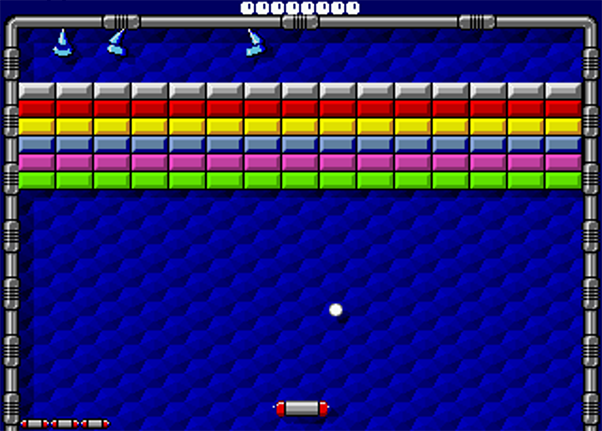
\includegraphics[width=0.6\textwidth]{img/arkanoid.png}
	\caption{Het 4de spel in de dataset}
	\label{fig:akranoid}
\end{figure}

\subsection{Logistische regressie}
\label{sec:Logistischeregressie-fase4}

Qua implementatie hoeft er niets te veranderen dus die blijft dezelfde als in code \ref{code:logistischeregressiefase3}. We gaan nu ook direct door naar de vijf inputparameters omdat die het meest aanleunen bij de realiteit. 

\subsubsection{Resultaten}
\paragraph{Snelheid van het algoritme} 
Het algoritme presteert na 29,8291 ms. Het is niet meer mogelijk om een foutloze hypothese te ontwikkelen en dus kijken we wanneer het algoritme het minst fouten maakt. Dit is nadat er 54 iteraties zijn gebeurd. Vanaf 64 iteraties worden er weer meer fouten gemaakt. Dit komt doordat de hypothese begint te overfitten dus niet meer goed generaliseert en daardoor zullen er sneller fouten gemaakt worden.
Wanneer het algoritme optimaal is, na 54 iteraties, maakt het algoritme slechts 3 fouten van de 200 voorbeelden.

\paragraph{Foutratio} 
Voor het foutratio meten we het aantal fouten wanneer de tolerance is ingesteld op 0,1. Dan behaalt het algoritme 181/200 wat nog altijd niet slecht is. Wat opvalt en ook wel te verwachten was is dat er 9 fouten van de 19 gebeuren tussen Pacman en Arkanoid. Als we kijken naar een foutieve voorspelling dan zagen we dat Arkanoid voorspeld was terwijl het Pacman moest zijn. Uiteraard zijn de ButtonPresses en JoystickMovements gelijkaardig voor de 2 spelletjes. Wanneer we kijken naar 'TotalTimeOfNoUseOfControls' zien we dat Pacman daar 4892 ms heeft. Wij weten dat het maximum 5000 ms is. Terwijl die 5000 ms bij Arkanoid ongeveer in de midden ligt. Zo kunnen we ons inbeelden waarom de computer Arkanoid gekozen heeft boven Pacman. 

\newpage
\subsection{Support Vector Machine}
\label{sec:supportvectormachineFase4}
De implementatie voor de Support Vector Machine blijft net als de logistische regressie dezelfde als in fase 3. De code kan u terugvinden in figuur \ref{code:svmFase3imp} op pagina \ref{code:svmFase3imp}.

\subsubsection{Resultaten}
\paragraph{Snelheid van het algoritme} 
De support vector machine haalt een gemiddelde van 169,4067 ms wanneer de complexity 100 is. Hoe hoger de complexity hoe preciezer de hypothese maar dus hoe slechter die generaliseert. 100 is een matige waarde hiervoor. Er zijn gemiddeld 9 fouten met een standaard afwijking van 3. We praten nu over gemiddeld aantal fouten omdat het leeralgoritme van de support vector machine stopt in een lokaal minimum.

\paragraph{Foutratio}
We verwijderen de complexity nu en de Tolerance zetten we op 0,1. Op die manier scoort de SVM 188/200. Wat opvalt is dat hier alle fouten gemaakt worden tussen Arkanoid en Pacman. 

\subsection{Conclusie na fase 4}
Nadat we een vierde spel hebben toegevoegd aan de dataset kunnen we duidelijkere conclusies trekken. Een eerste duidelijk verschil bevindt zich in de snelheid. Wanneer we de algoritmen naar hun optimale resultaat dwingen is logistische regressie 5,6 keer sneller dan een support vector machine. Ook de resultaten van het geoptimaliseerde algoritme waren in het voordeel van logistische regressie. 

De foutratio's van beide algoritmen verschillen niet zo super veel. We merken wel dat de support vector machine het toch beter doet dan logistische regressie. Wanneer de fouten onderzocht werden viel het op dat de SVM enkel fouten maakten tussen Pacman en Arkanoid. terwijl logistische regressie nog 10 fouten maakte op de andere klassen, Tetris en Mortal Kombat. 

 